\documentclass[9,aspectratio=169]{beamer}

%\usetheme[secheader]{Boadilla}
\usetheme{CambridgeUS}
%usecolortheme{seahorse}
\usepackage[utf8]{inputenc}
\usepackage{comment}
\usepackage{amsmath}
\usepackage{amssymb}
\usepackage{graphicx}
\usepackage{subfigure}
\usepackage{appendixnumberbeamer}
\usepackage{verbatim}
\usepackage{nicefrac}
\definecolor{links}{HTML}{2A1B81}
\usepackage{tikz}
\usetikzlibrary{arrows,shapes}
\setbeamertemplate{blocks}[rounded][shadow=true]
\setbeamertemplate{navigation symbols}{}
\newcommand{\pt}{\ensuremath{p_{\mathrm{T}}}}
\newcommand{\mt}{\ensuremath{m_{\mathrm{T}}}}
\newcommand{\ptAnd}[1]{\ensuremath{p_{\mathrm{T},#1}}}
\newcommand{\Mjj}{\ensuremath{M_{\mathrm{jj}}}}
\newcommand{\kt}{\ensuremath{k_{\mathrm{T}}}}
\newcommand{\antikt}{anti-\kt}
\newcommand{\abs}[1]{\left|#1\right|}
\newcommand{\largeInt}[2]{\mathlarger{\int\limits^{#2}_{#1}}}
\newcommand{\pythia}{\textsc{Pythia}}
\newcommand{\jewel}{\textsc{Jewel}}
\newcommand{\hepmc}{\textsc{HepMC}}
\newcommand{\fastjet}{\textsc{FastJet}}
\newcommand{\powheg}{\textsc{Powheg}}
\newcommand{\geant}{\textsc{Geant}}
\newcommand{\roounfold}{\textsc{RooUnfold}}
\newcommand{\dd}{\mathrm{d}}
\newcommand{\snn}{\ensuremath{\sqrt{s_\mathrm{NN}}}}
\newcommand{\RAA}{\ensuremath{R_\mathrm{AA}}}

\include{hyperref}

\graphicspath{{Figures/}}

% Main page
\title[ToyFlow]{\bf{ToyFlow MC tool for FIT}}
%\subtitle{Correlation in ALICE at LHC}
\vspace{\fill}
\vspace{\fill}
\author[Rytk\"onen, Saarim\"aki and R\"as\"anen]{{\bf Heidi Rytk\"onen, Oskari Saarim\"aki and Sami R\"as\"anen} }
%{\small Dongjo Kim, Beomkyu Kim, Tomas Snellman, Sami R\"as\"anen}}
%author{\makebox[.9\textwidth]{Lead Author}\\Dept\\ School \and Co-Author1\\Dept\\ School \and Co-Author2\\Dept\\ School \and Co-Author3\\Dept\\ School}
\institute[JYFL/HIP]{University of Jyv\"askyl\"a \\
\& Helsinki Institute of Physics}
\date{}

\begin{document}


\frame[noframenumbering]{\titlepage
    \thispagestyle{empty}
    \begin{center}
        \small \today
    \end{center}
    \begin{figure}[ht]
        \begin{center}
            
\includegraphics[width=0.21\textwidth]{logo_jyu}\hspace{3em}
\includegraphics[height=1.6cm]{logo_alice.eps}\hspace{3em}
            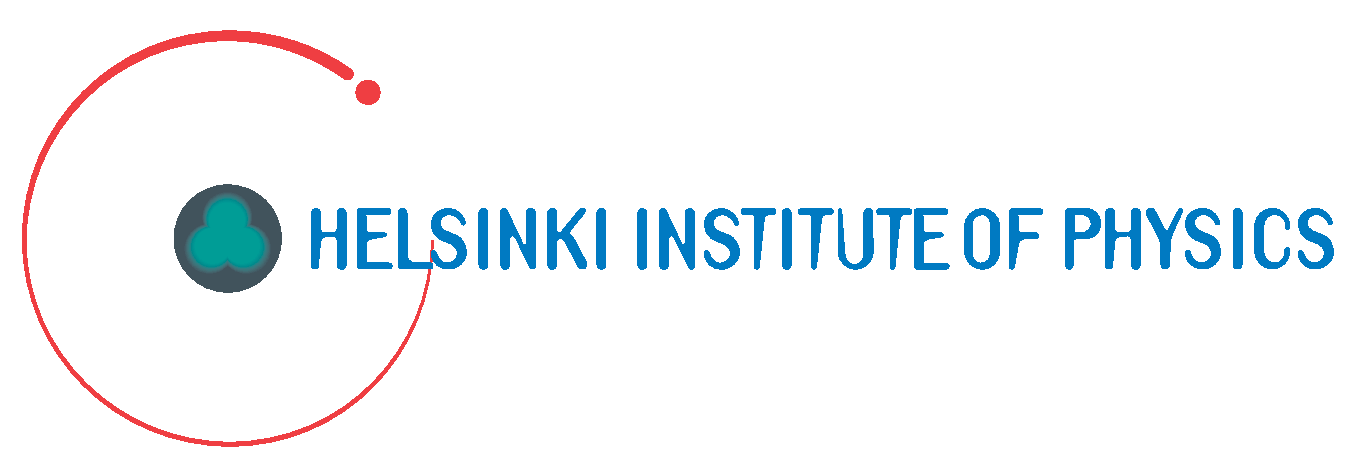
\includegraphics[width=0.21\textwidth]{logo_hip}
            %PLHC 2012 - Physics at the LHC 2012, Vancouver June 4-9

        \end{center}
    \end{figure}

}

\frame {
    \frametitle{Introductions}
    \begin{columns}
        \column{.2\textwidth}
        \begin{figure}[htbp]
            \includegraphics[width=0.70\textwidth]{Persons/Heidi.jpeg}
        \end{figure}
        \column{.8\textwidth}
        Heidi Rytkönen
        \begin{itemize}
            \item PhD. student
        \end{itemize}
    \end{columns}
    \vfill
    \begin{columns}
        \column{.2\textwidth}
        \begin{figure}[htbp]
            \includegraphics[width=0.70\textwidth]{Persons/Oskari.jpeg}
        \end{figure}
        \column{.8\textwidth}
        Oskari Saarimäki
        \begin{itemize}
            \item PhD. student
        \end{itemize}
    \end{columns}
}

\frame {
    \frametitle{Introductions}
    \begin{columns}
        \column{.2\textwidth}
        \begin{figure}[htbp]
            \includegraphics[width=0.70\textwidth]{Persons/DongJo.jpeg}
        \end{figure}
        \column{.3\textwidth}
        Dong Jo Kim
        \begin{itemize}
            \item Senior researcher
            \item Flow expert
        \end{itemize}
        \column{.2\textwidth}
        \begin{figure}[htbp]
            \includegraphics[width=0.70\textwidth]{Persons/Sami.jpg}
        \end{figure}
        \column{.3\textwidth}
        Sami Räsänen
        \begin{itemize}
            \item Senior researcher
            \item Supervisor
        \end{itemize}
    \end{columns}
    \vfill
    \begin{columns}
        \column{.2\textwidth}
        \begin{figure}[htbp]
            \includegraphics[width=0.70\textwidth]{Persons/Jasper.jpeg}
        \end{figure}
        \column{.8\textwidth}
        Jasper Parkkila
        \begin{itemize}
            \item PhD. student
            \item Flow expert
        \end{itemize}
    \end{columns}
}



\frame {
    \frametitle{Motivation}
    \begin{columns}
        \column{.70\textwidth}
        \begin{itemize}
            \item The particle azimuthal distribution is not isotropic.
            \item It is customary to expand it in a Fourier series:
            \begin{equation} \small\nonumber
                E\frac{\dd^3N}{\dd^3p} \propto 1+\sum^\infty_{n=1}2v_n\cos\left(n\left(\phi-\Psi_\mathrm{RP}\right)\right)
            \end{equation}
            where
            \begin{equation} \small\nonumber
                v_n = \left\langle\cos\left[n\left(\phi_i-\Psi_\mathrm{RP}\right)\right]\right\rangle
            \end{equation}
            and angled brackets mean an average over all particles in all events.
        \end{itemize}
        \column{.30\textwidth}
        \begin{figure}[htbp]
            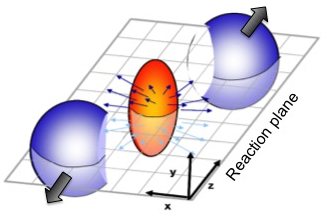
\includegraphics[width=0.95\textwidth]{toyFlow/flow2.jpg}
        \end{figure}
    \end{columns}
}

\frame {
    \frametitle{Event plane}
    \begin{columns}
        \column{.70\textwidth}
        \begin{itemize}
            \item Problem: $\Psi_\mathrm{RP}$ is unknown when using real data.
            \item Define the event flow vector $\mathbf{Q_n} \in \mathbb{C}$:
            \begin{equation} \small
                \mathbf{Q}_n = w_i e^{in\Psi_n}
            \end{equation}
            where $w_i$ are the weights and optimally $w_i\approx v_n\left(\pt,y\right)\propto\pt$, with small \pt. Many times it is set $w_i=1$ for all $i$.
        \end{itemize}
            \begin{equation} \small
                \Psi_n = \frac{1}{n}\arctan\left(\frac{Q_{n,y}}{Q_{n,x}}\right) \nonumber
            \end{equation}
        \begin{itemize}
            \item Now we have
            and now the observed $v_n$ can be calculated using
                \begin{equation}
                v_n^\mathrm{obs} = \left\langle\cos\left[n\left(\phi_i-\Psi_n\right)\right]\right\rangle \nonumber
            \end{equation}
        \end{itemize}
        \column{.30\textwidth}
        \begin{figure}[htbp]
            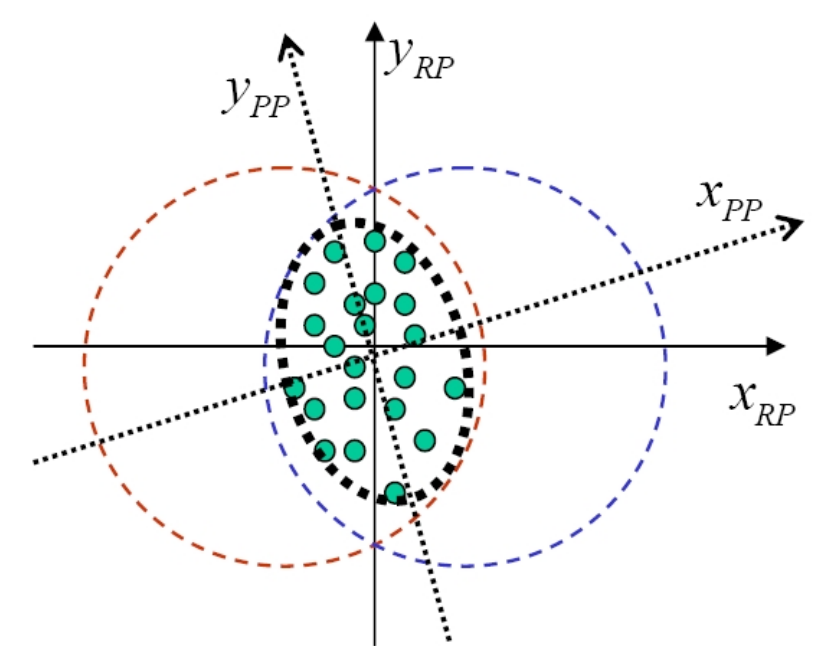
\includegraphics[width=0.95\textwidth]{toyFlow/reaction-plane-yms.png}
            \caption{From arXiv:0809.2949v2}
        \end{figure}
    \end{columns}
}

\frame {
    \frametitle{Event plane}
    \begin{columns}
        \column{.70\textwidth}
            A resolution parameter is defined
            \begin{equation}
                R_{n,true} = \left\langle\cos\left[n\left(\Psi_n-\Psi_\mathrm{RP}\right)\right]\right\rangle, \nonumber
            \end{equation}
            so that
            \begin{equation}
                v_n = \frac{v_n^\mathrm{obs}}{R_{n,true}}. \nonumber
            \end{equation}
            The above definition of $R_n$ can only be used with simulations as the $\Psi_\mathrm{RP}$ is unknown, but it can also be evaluated without the information of reaction plane by using subevents A and B.
        \column{.30\textwidth}
        \begin{figure}[htbp]
            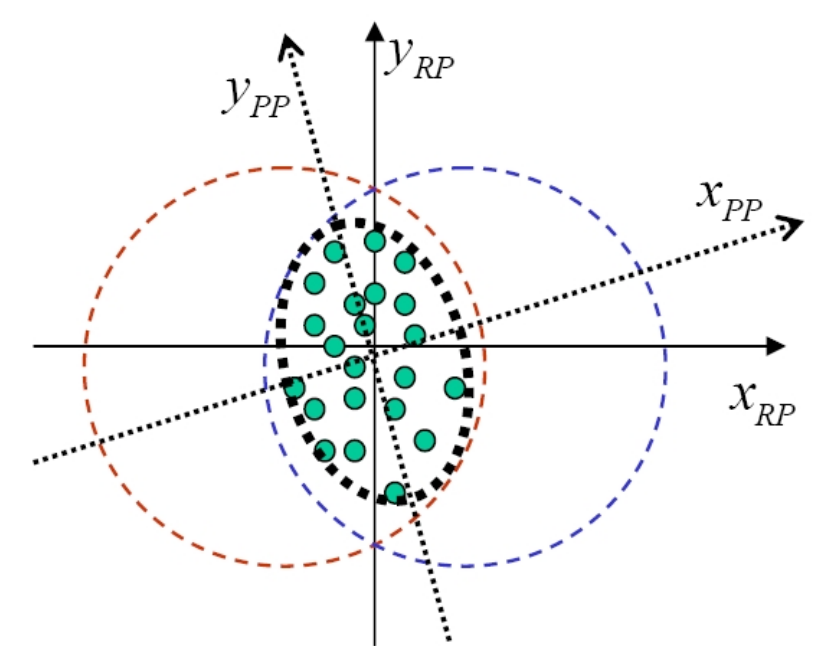
\includegraphics[width=0.95\textwidth]{toyFlow/reaction-plane-yms.png}
            \caption{From arXiv:0809.2949v2}
        \end{figure}
    \end{columns}
}

\frame {
    \frametitle{Toy Monte Carlo}
    \begin{columns}
        \column{1.0\textwidth}
        \begin{itemize}
            \item Toy MC to study the resolution parameter and flow coefficients
            \item Uses measured data for $v_{\text{n}}$ and $\eta$-distribution from \href{https://arxiv.org/abs/1804.02944}{arXiv:1804.02944} and \href{https://arxiv.org/abs/1509.07299}{arXiv:1509.07299} respectively
            \item Code available at \url{https://github.com/hrytkone/ToyFlow}
        \end{itemize}
    \end{columns}
}

\frame {
    \frametitle{How the event is formed}
    \begin{columns}
        \column{.5\textwidth}
        \begin{itemize}
            \item Event multiplicity taken from data according to centrality
            \item Then for each particle in the event
            \begin{itemize}
                \item $\phi$ is taken from the Fourier series
                \item $\eta$ is taken from multiplicity distribution
            \end{itemize}
        \end{itemize}
        \column{.5\textwidth}
        \begin{figure}[htbp]
            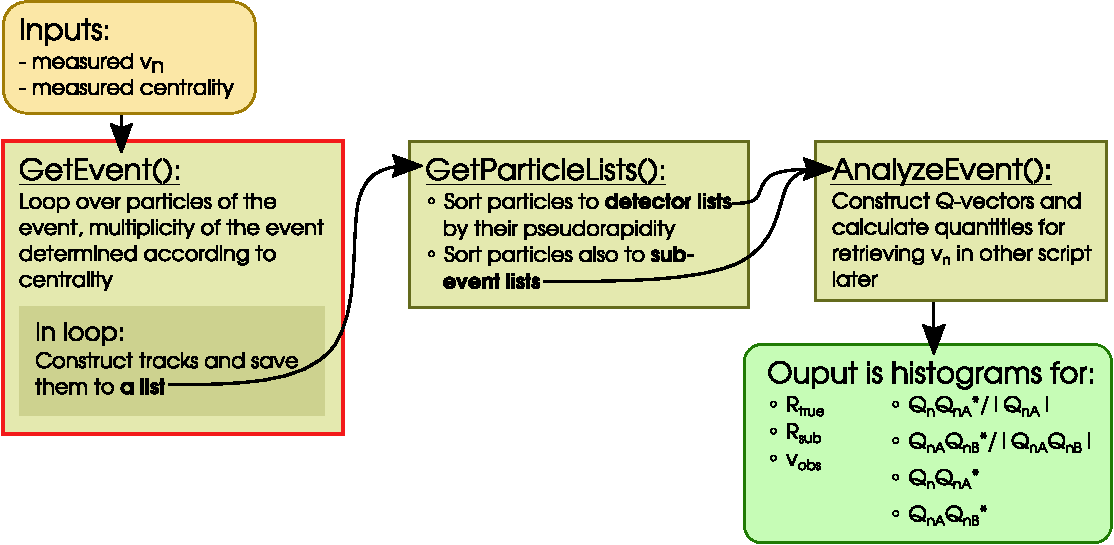
\includegraphics[width=0.95\textwidth]{Figures/toyFlow_chart_3.pdf}
        \end{figure}
    \end{columns}
}

\frame {
    \frametitle{How the event is formed}
    \begin{columns}
        \column{.5\textwidth}
        \begin{itemize}
            \item Particles in full event are divided into detector specific lists according to pseudorapidity
            \begin{itemize}
                \item Detectors are TPC, FT0-A, FT0-C and FV0
            \end{itemize}
            \item Particles are also divided into two sub events
        \end{itemize}
        \column{.5\textwidth}
        \begin{figure}[htbp]
            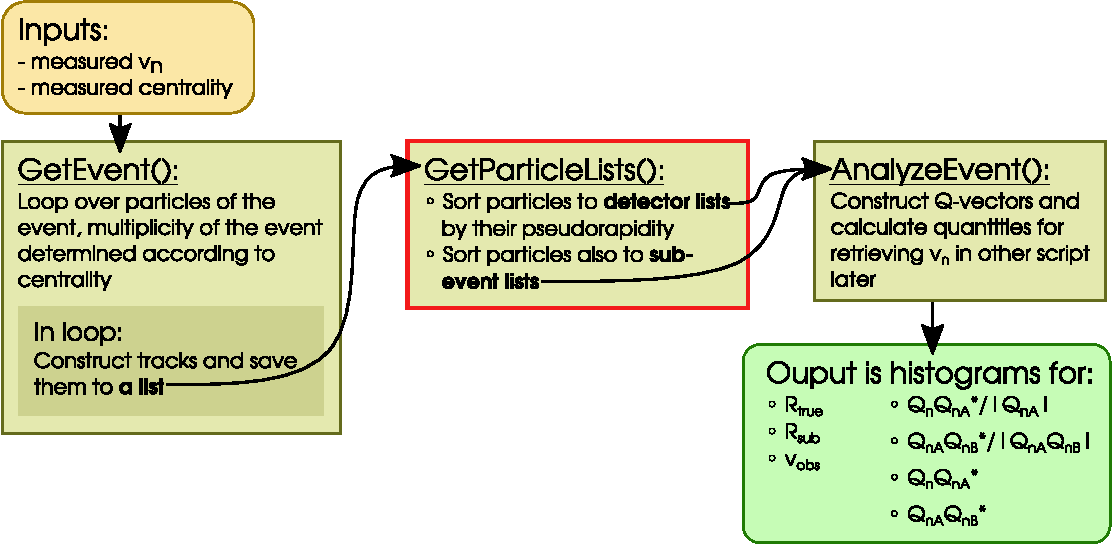
\includegraphics[width=0.95\textwidth]{Figures/toyFlow_chart_4.pdf}
        \end{figure}
    \end{columns}
}

\frame {
    \frametitle{How the event is formed}
    \begin{columns}
        \column{.5\textwidth}
        \begin{itemize}
            \item Q-vectors are then calculated
            \item Relevant information for retrieving the flow coefficients is saved to the histograms
        \end{itemize}
        \column{.5\textwidth}
        \begin{figure}[htbp]
            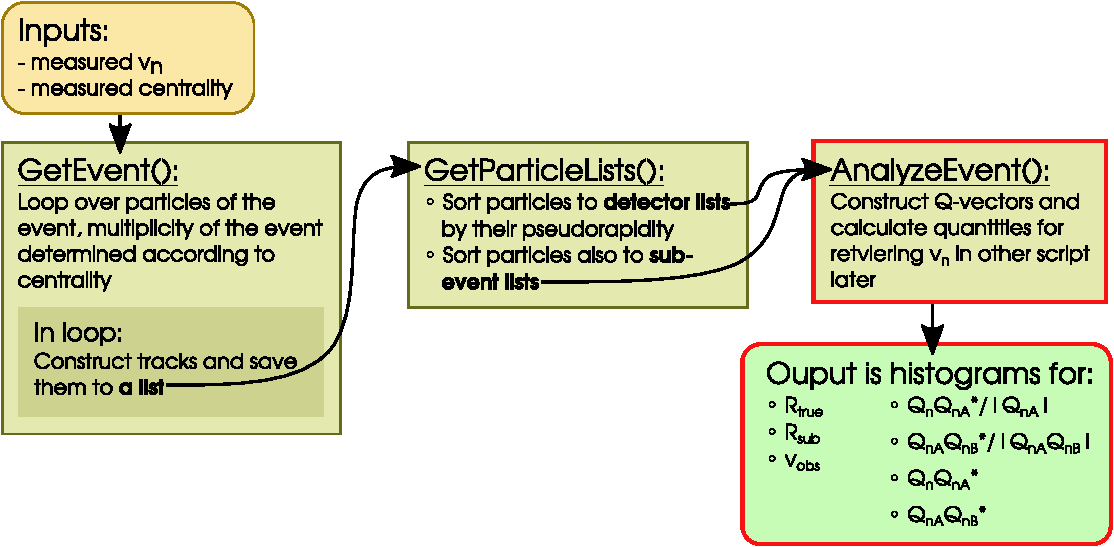
\includegraphics[width=0.95\textwidth]{Figures/toyFlow_chart_5.pdf}
        \end{figure}
    \end{columns}
}

\frame {
    \frametitle{Validating}
        \begin{figure}[htbp]
            \begin{itemize}
                \item In ideal situation the code produces the flow coefficients $v_2$ and $v_3$ well
            \end{itemize}
            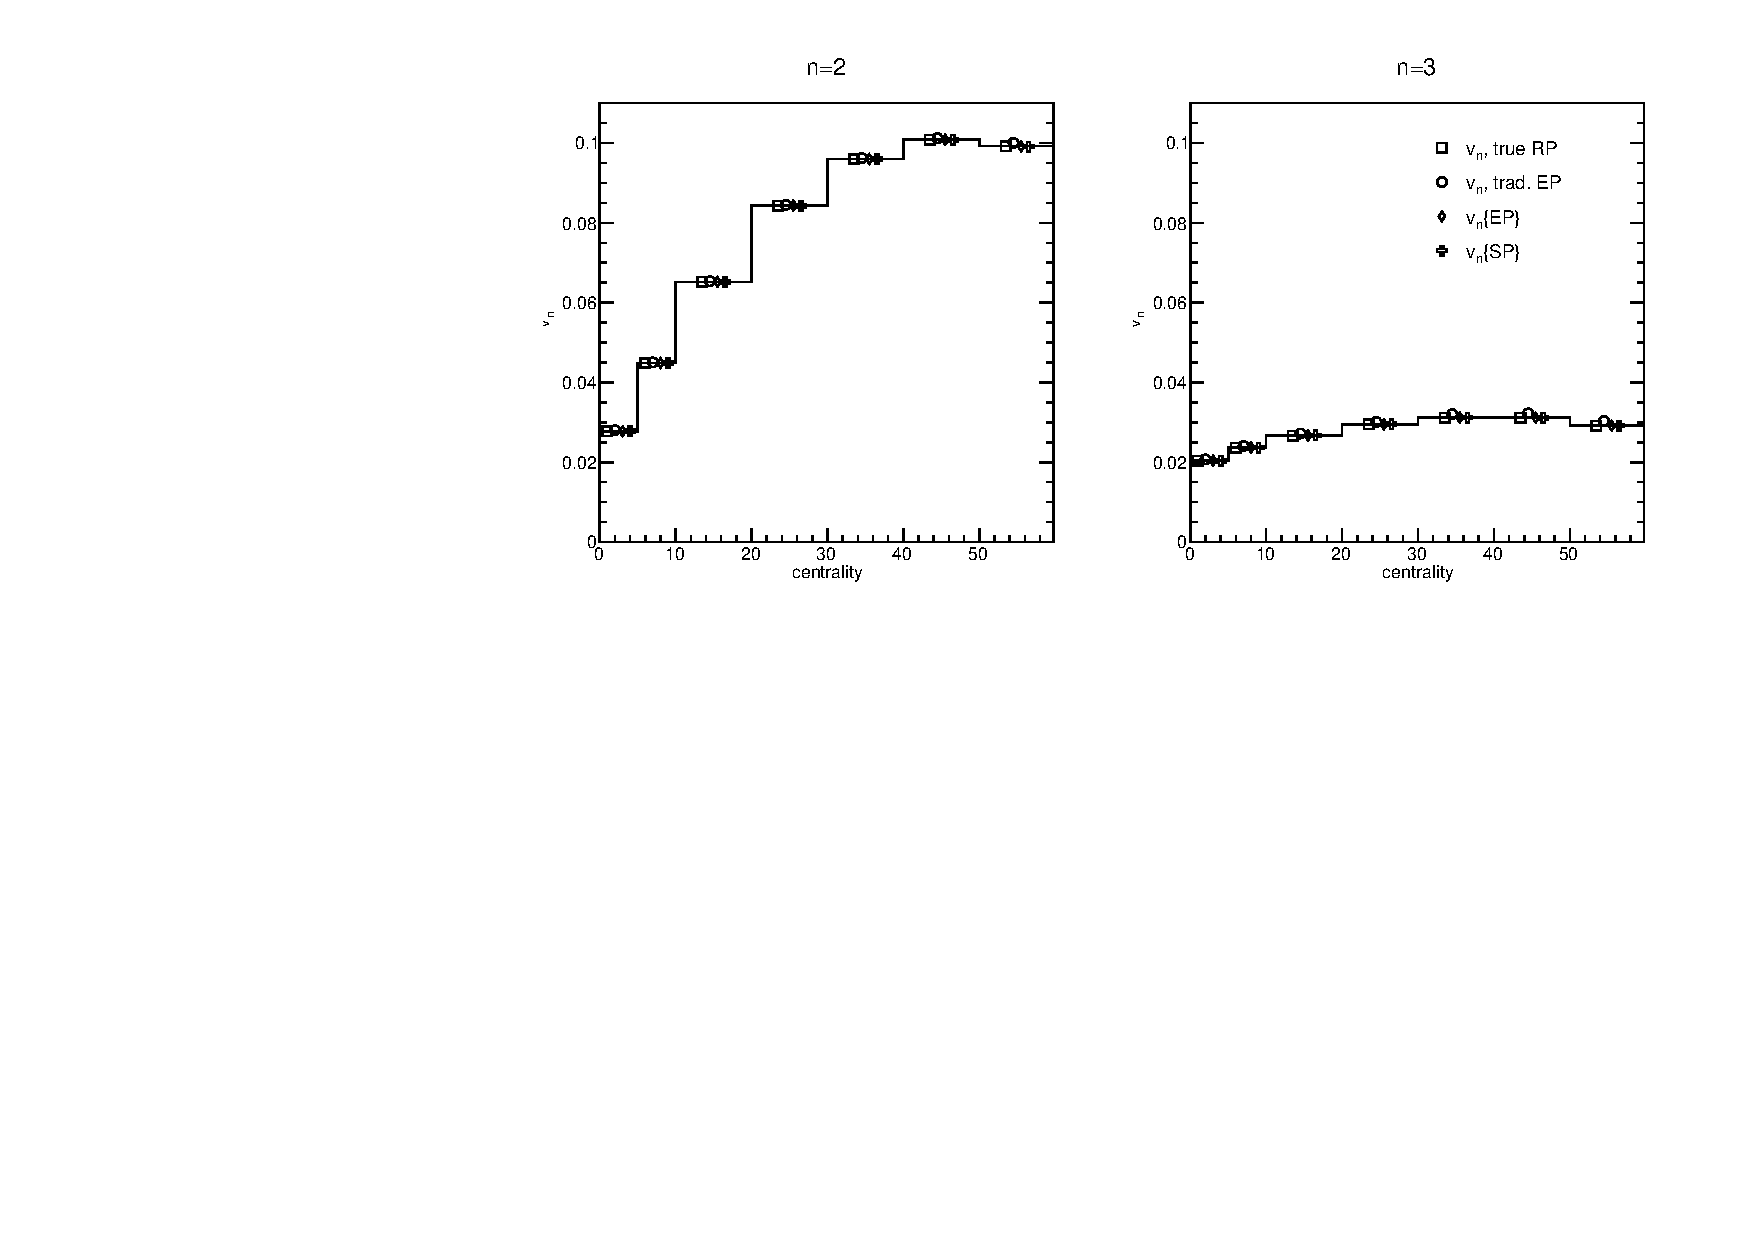
\includegraphics[width=0.85\textwidth]{FIT-vn-ideal.pdf}
            \caption{}
        \end{figure}
}

\frame {
    \frametitle{Validating (if needed)}
        \begin{figure}[htbp]
            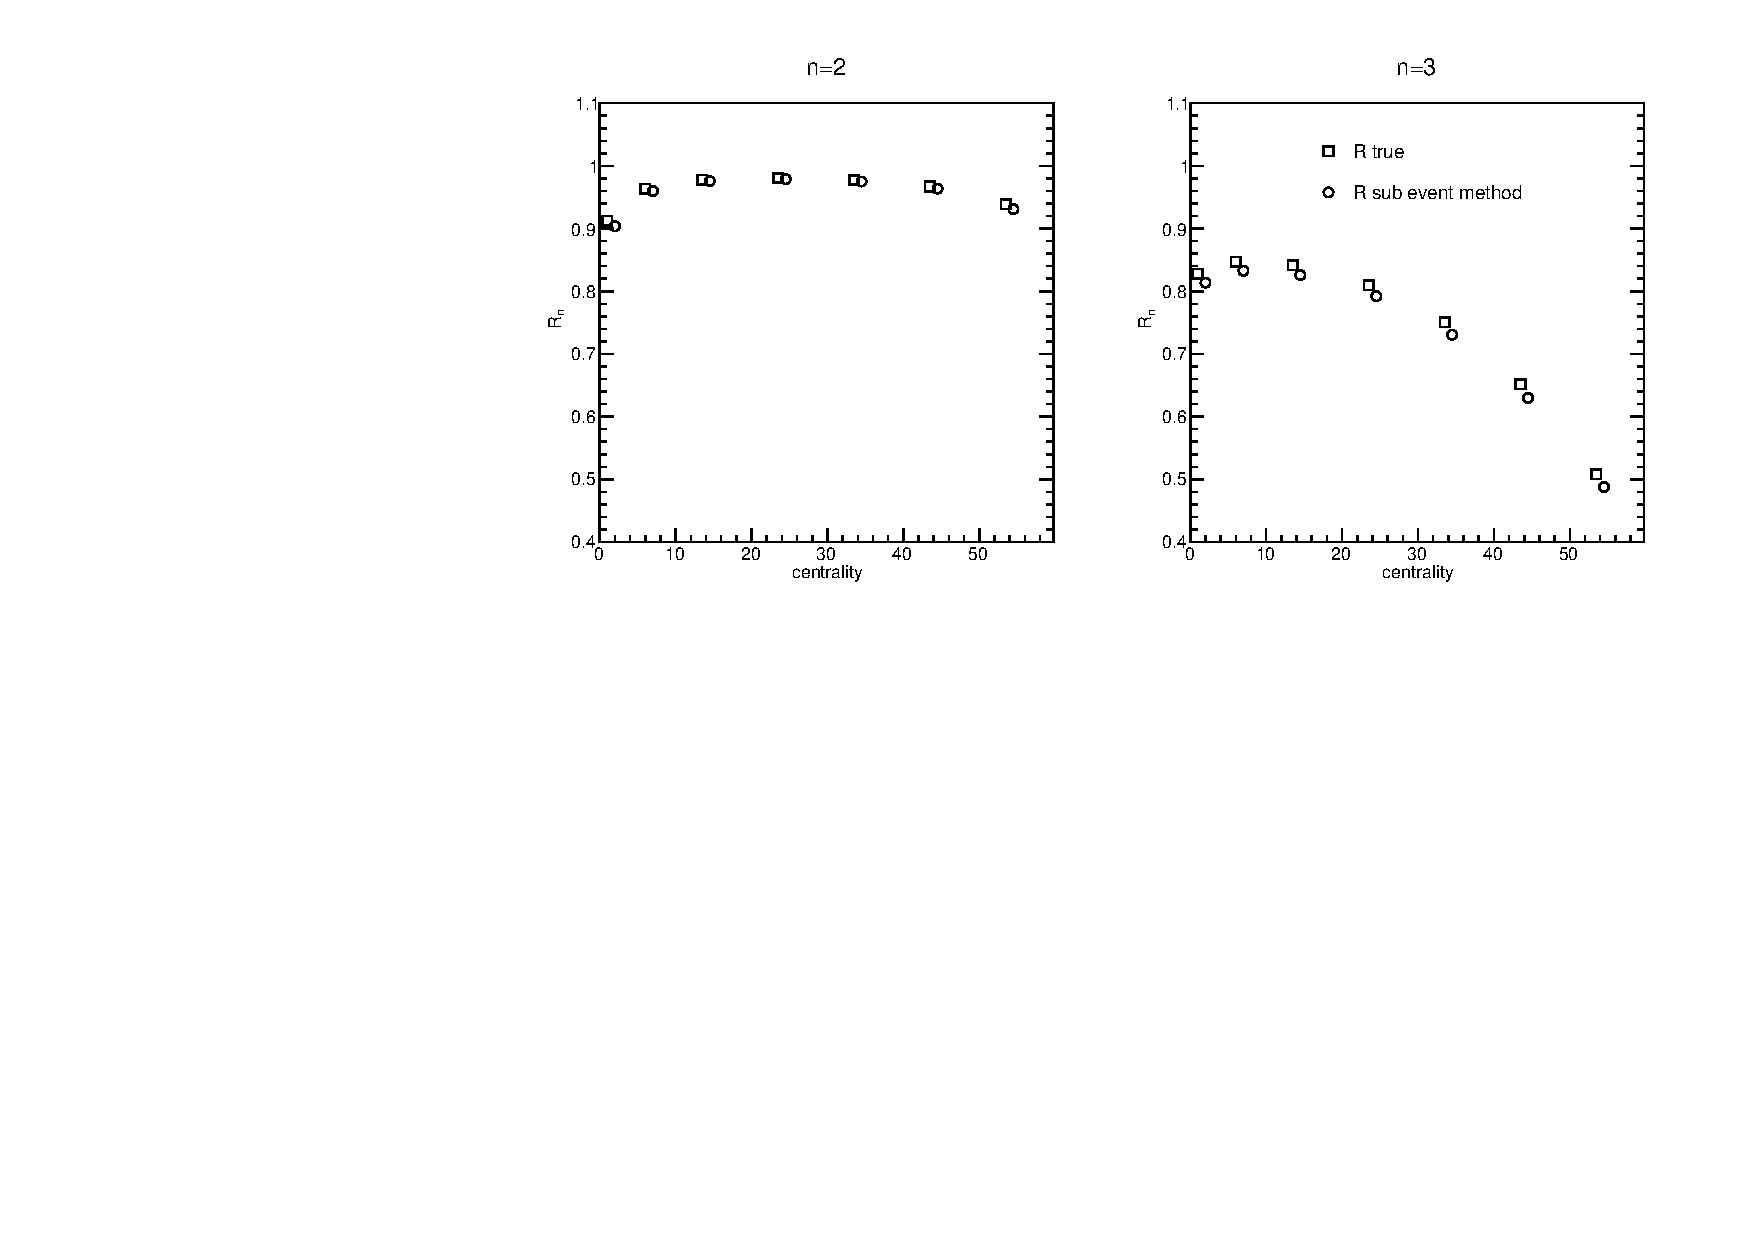
\includegraphics[width=0.95\textwidth]{FIT-Rn-ideal.pdf}
            \caption{}
        \end{figure}
}

\frame {
    \frametitle{Validating}
        \begin{figure}[htbp]
            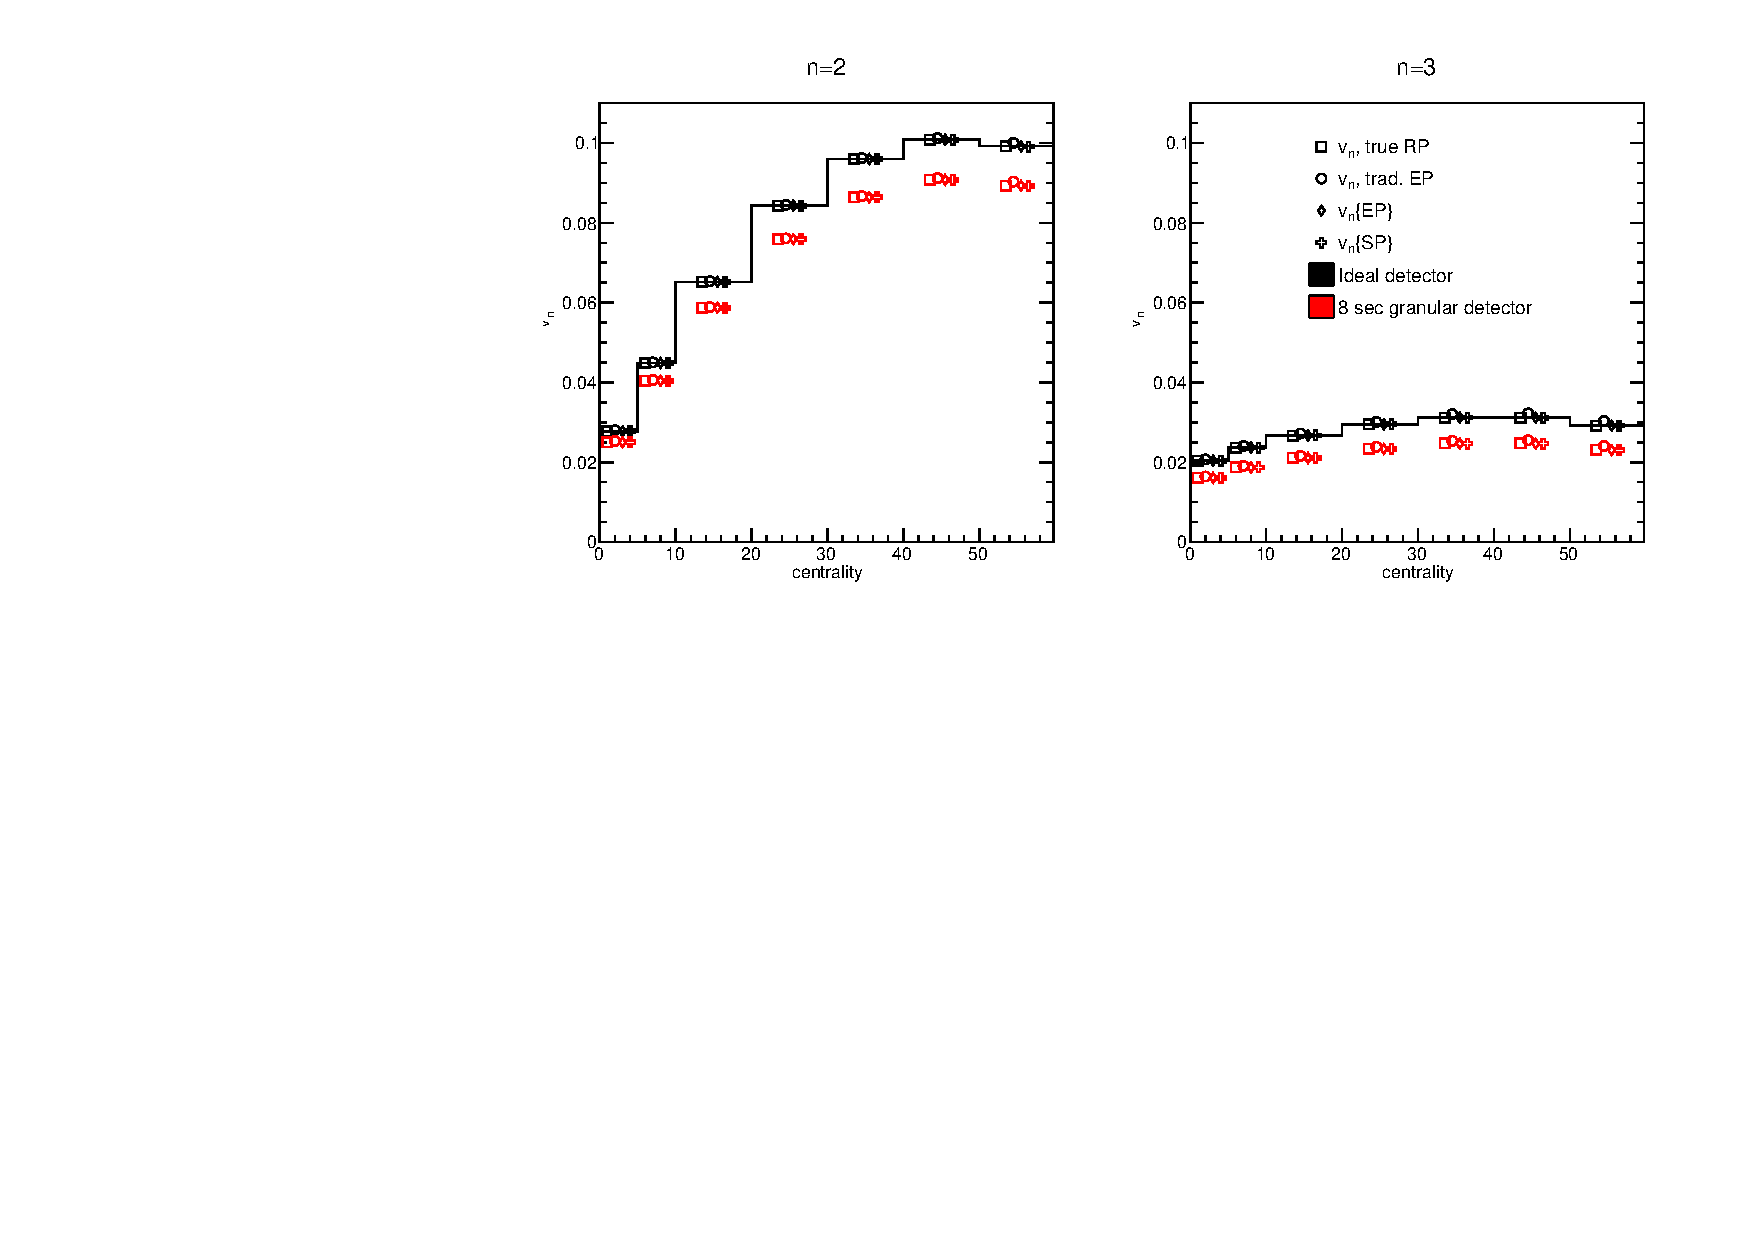
\includegraphics[width=0.95\textwidth]{FIT-vn-multiple.pdf}
            \caption{}
        \end{figure}
}

\frame {
    \frametitle{Validating (if needed)}
        \begin{figure}[htbp]
            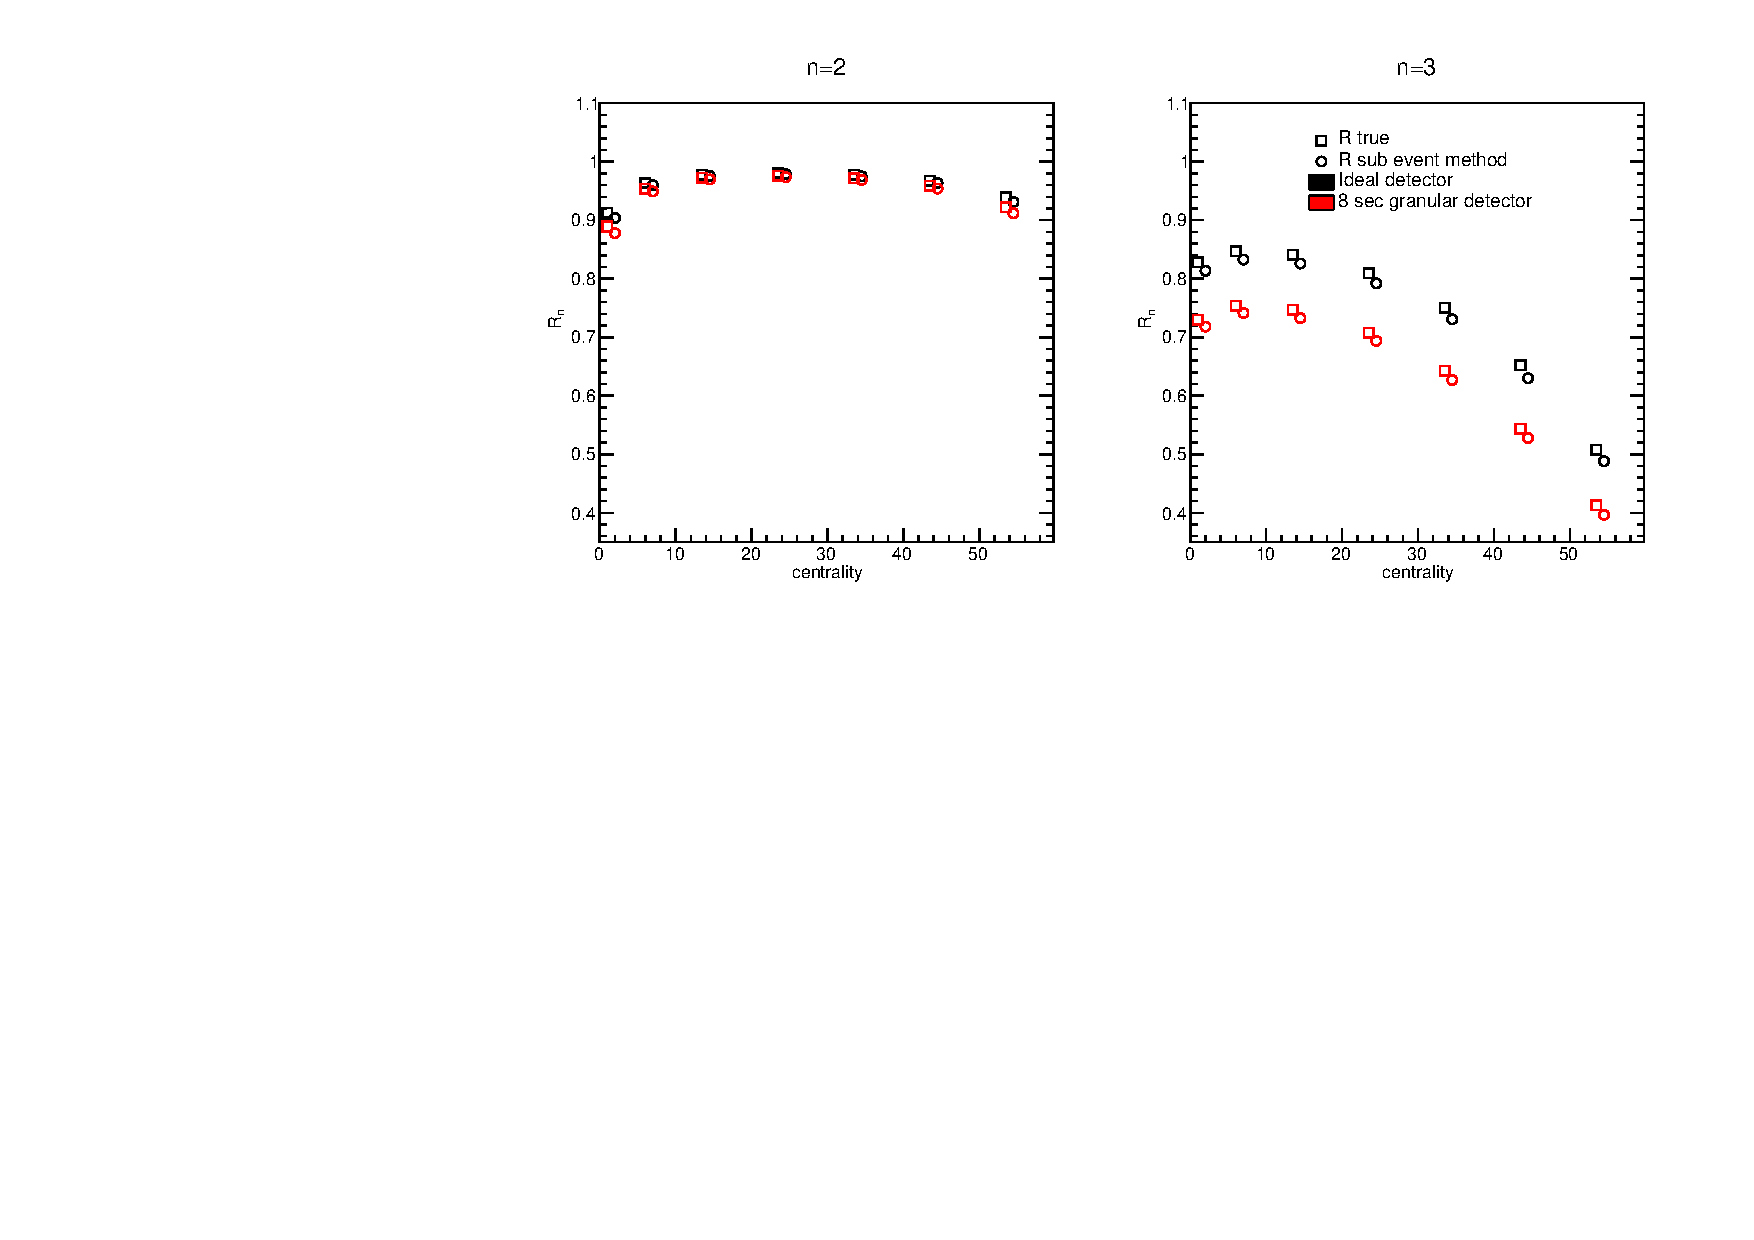
\includegraphics[width=0.95\textwidth]{FIT-Rn-multiple.pdf}
            \caption{}
        \end{figure}
}

\frame {
    \frametitle{Simulations using FV0}
    \begin{columns}
        \column{0.5\textwidth}
        \begin{itemize}
            \item Ideal vs. gran
            \item Compare to Maciej:\\ \url{https://indico.cern.ch/event/703569/contributions/2886293/attachments/1597688/2531598/2018.02.08-Slupecki-ToyFlow.pdf}
        \end{itemize}
        \column{0.5\textwidth}
        \begin{figure}[htbp]
            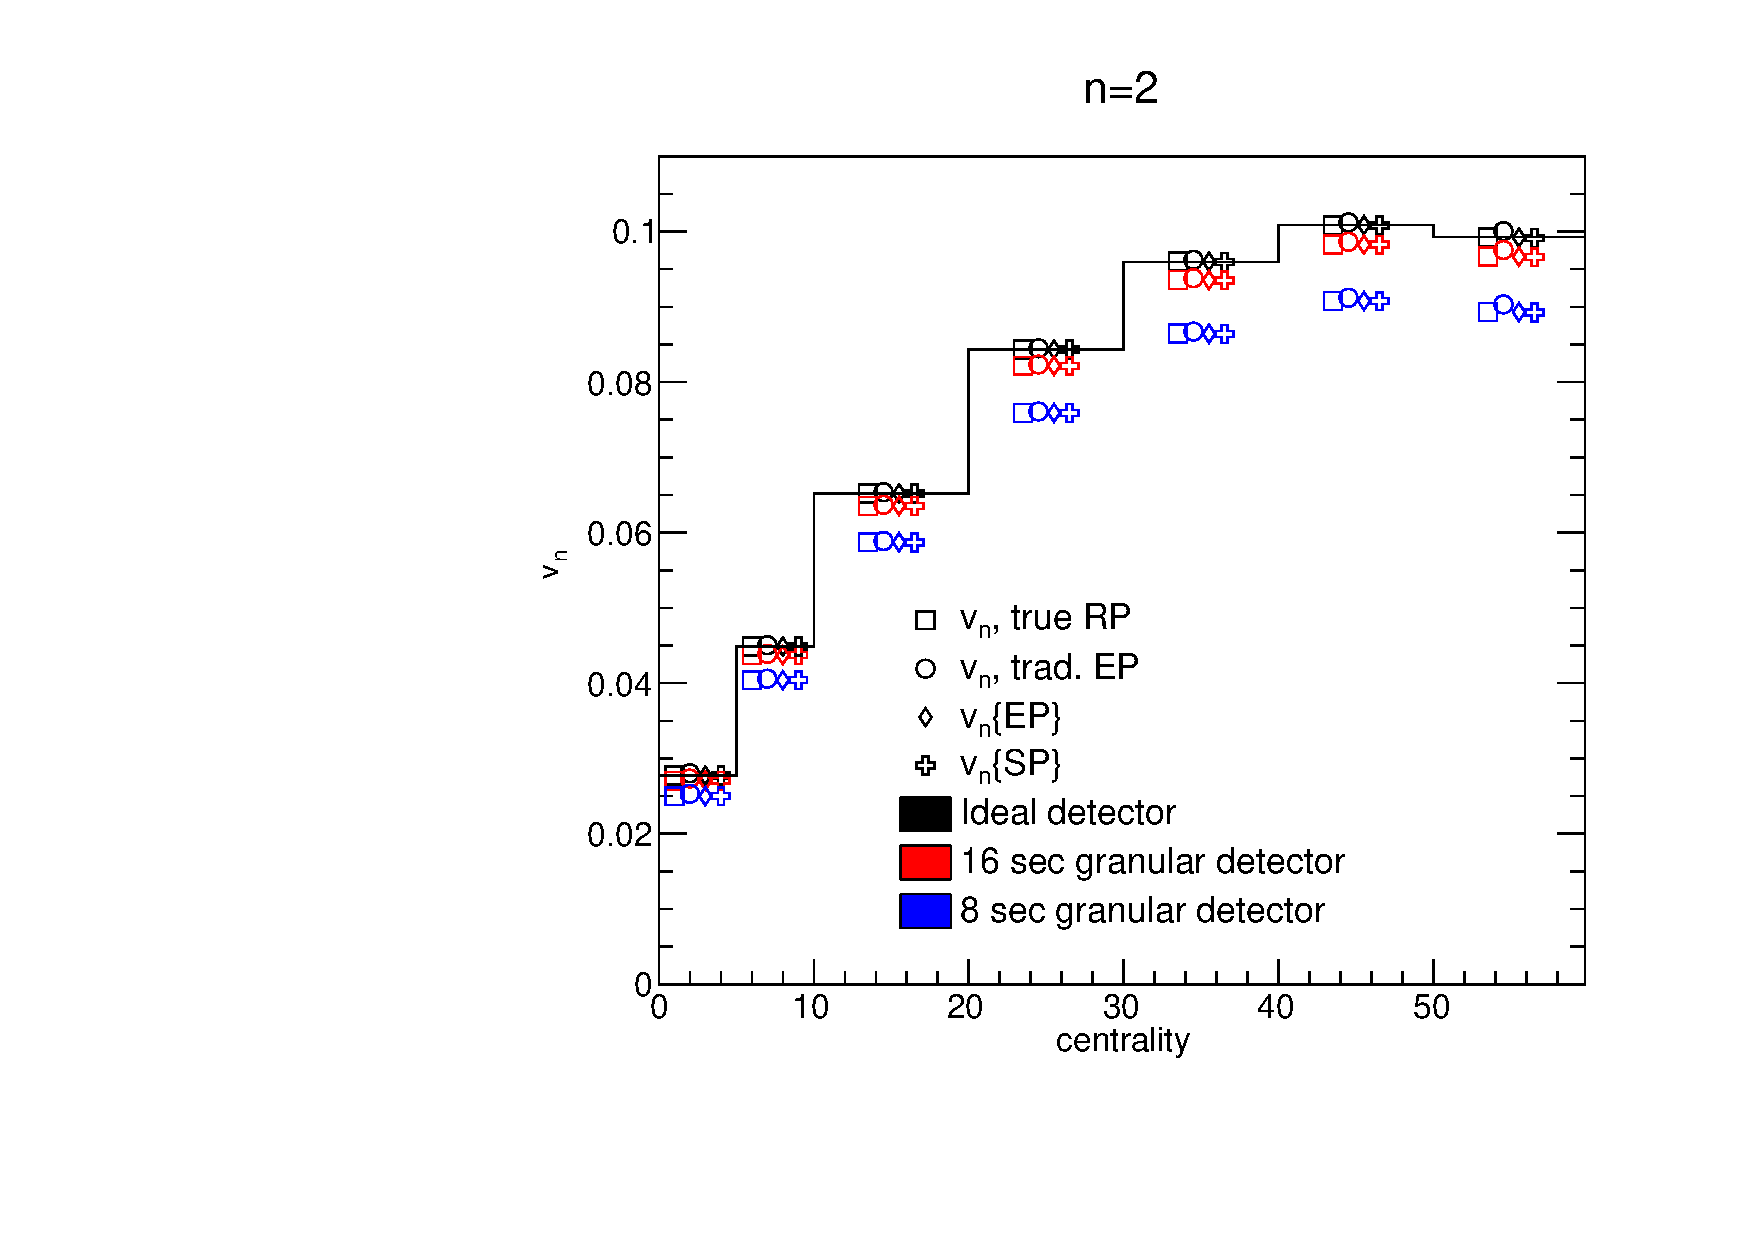
\includegraphics[width=0.5\textwidth]{FIT-vn-single.pdf}
        \end{figure}
    \end{columns}
}

\frame {
    \frametitle{TODO}
    \begin{columns}
        \column{1.0\textwidth}
        \begin{itemize}
            \item TODO:
            \begin{itemize}
                \item Subevent handling
                \begin{itemize}
                    \item In FIT?
                \end{itemize}
                \item Realistic geometry.
            \end{itemize}
            \item In the future:
            \begin{itemize}
                \item Realistic simulation of FIT.
            \end{itemize}
        \end{itemize}
    \end{columns}
}

\frame{
    %\thispagestyle{empty}
    \frametitle{The end}
    \centering
    \vfill
    {\LARGE Thank you for listening}
    \vspace{3em}

    Questions?
    \vspace{9em}

    %{\small Next some extra pages}
}

\appendix

\frame {
    \frametitle{Event plane}
    \begin{columns}
        \column{.70\textwidth}
        \begin{itemize}
            \item $R_n$ can also be written as
            \begin{equation} \small
                R_k \left(\chi\right)= \frac{\sqrt{\pi}}{2}\chi e^{-\frac{\chi^2}{2}} \left[I_\frac{k-1}{2}\left(\frac{\chi^2}{2}\right) + I_\frac{k+1}{2}\left(\frac{\chi^2}{2}\right)\right], \nonumber
            \end{equation}
            where $I$ is the modified Bessel function and
            \begin{equation}
                \chi = v_n\sqrt{M} \nonumber
            \end{equation}
            where $M$ is the multiplicity of the event. When comparing the same harmonic number correlation and event plane, $k=1$ always.
        \end{itemize}
        \column{.30\textwidth}
        \begin{figure}[htbp]
            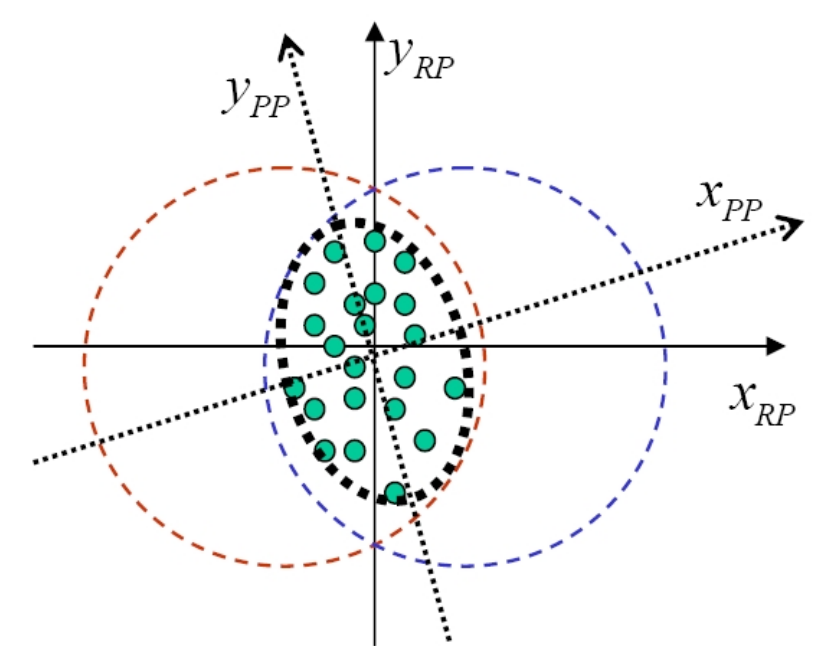
\includegraphics[width=0.95\textwidth]{toyFlow/reaction-plane-yms.png}
            \caption{From arXiv:0809.2949v2}
        \end{figure}
    \end{columns}
}

\frame {
    \frametitle{Event plane}
    \begin{columns}
        \column{.70\textwidth}
        \begin{itemize}
            \item By splitting the event into two equal size independent sub-events
            \begin{equation} \small
                R_{n,sub} = \sqrt{\left\langle\cos\left[n\left(\Psi_n^\mathrm{A}-\Psi_n^\mathrm{B}\right)\right]\right\rangle}, \nonumber
            \end{equation}
            and then $\chi_\mathrm{sub}$ can be solved iteratively from the previous page equation.
            \item Because $\chi\propto\sqrt{M}$, the full event $\chi = \sqrt{2}\,\chi_\mathrm{sub}$, and so finally full event resolution
            \begin{equation}
                R_{n} = R_{k=1}\left(\chi\right) \nonumber
            \end{equation}
            and
            \begin{equation}
                v_n = \frac{v_n^\mathrm{obs}}{R_n} \nonumber
            \end{equation}
        \end{itemize}
        \column{.30\textwidth}
        \begin{figure}[htbp]
            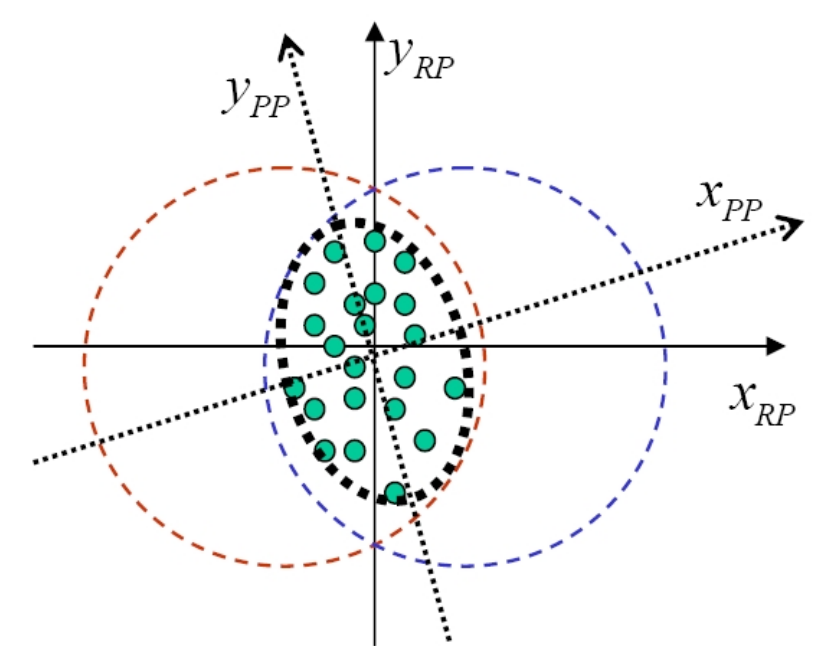
\includegraphics[width=0.95\textwidth]{toyFlow/reaction-plane-yms.png}
            \caption{From arXiv:0809.2949v2}
        \end{figure}
    \end{columns}
}

\frame {
    \frametitle{Event plane}
    \begin{columns}
        \column{.70\textwidth}
        \begin{itemize}
            \item Summary table:
                \begin{table}[tb]
                    \centering
                    \caption{Is possible to use.} \label{tab}
                    \begin{tabular}{ccc}
                        \hline
                        & Simulation & Data \\ \hline
                        $\Psi_\mathrm{RP}$ & x &  \\
                        $\Psi_n$ & x & x \\
                        $R_{n,true}$ & x &  \\
                        $R_n$ & x & x \\
                        \hline
                    \end{tabular}
                \end{table}
            \item When using a simulation the methods can be validated by comparing to the true values of reaction plane and $R_{n,true}$.
        \end{itemize}
        \column{.30\textwidth}
        \begin{figure}[htbp]
            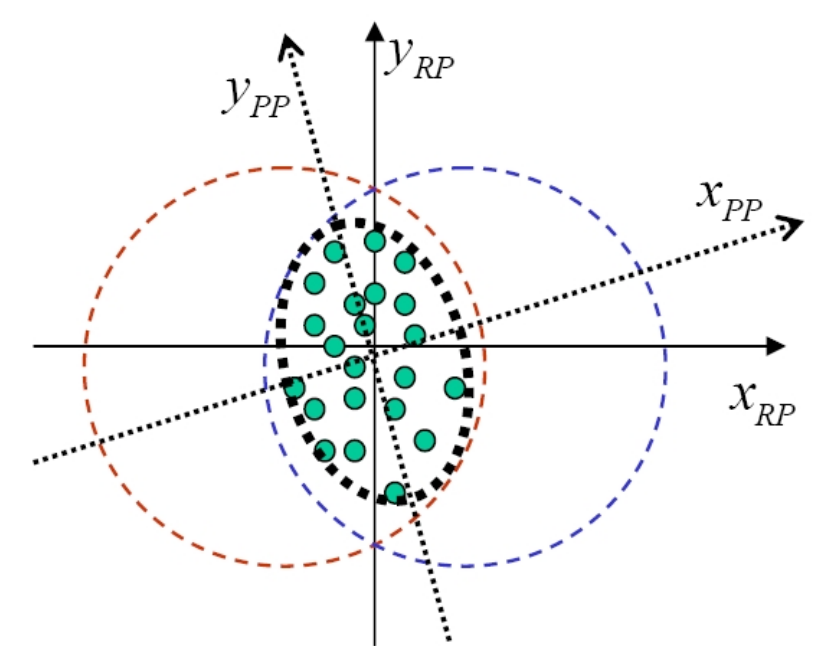
\includegraphics[width=0.95\textwidth]{toyFlow/reaction-plane-yms.png}
            \caption{From arXiv:0809.2949v2}
        \end{figure}
    \end{columns}
}

\frame {
    \frametitle{Event Plane (Scalar Product) method}
        \begin{itemize}
            \item Another way to calculate $v_n$:
            \begin{equation}
                \left\langle \mathbf{Q_n} \frac{\mathbf{Q_{n,A}}^*}{\abs{\mathbf{Q_{n,A}}}}\right\rangle = \left\langle \mathbf{Q_n} e^{-in\Psi_n}\right\rangle \left\langle\frac{\mathbf{Q_{n,A}}}{\abs{\mathbf{Q_{n,A}}}} e^{-in\Psi_n}\right\rangle^* = v_n R_{n,\mathrm{A}} \nonumber
            \end{equation}
            where the last equality is valid when $\mathbf{Q_n}$ and $\mathbf{Q_{n,A}}$ are uncorrelated, except for the common $\Psi_n$.
            \item For two subevents with equal multiplicities
            \begin{equation}
                \left\langle \frac{\mathbf{Q_{n,A}}}{\abs{\mathbf{Q_{n,A}}}} \frac{\mathbf{Q_{n,B}}^*}{\abs{\mathbf{Q_{n,B}}}}\right\rangle = \left\langle\frac{\mathbf{Q_{n,A}}}{\abs{\mathbf{Q_{n,A}}}} e^{-in\Psi_n}\right\rangle \left\langle\frac{\mathbf{Q_{n,B}}}{\abs{\mathbf{Q_{n,B}}}} e^{-in\Psi_n}\right\rangle^* = \abs{\left\langle\frac{\mathbf{Q_{n,A}}}{\abs{\mathbf{Q_{n,A}}}} e^{-in\Psi_n}\right\rangle}^2 = R_{n,\mathrm{A}}^2 \nonumber
            \end{equation}
            \item The scalar product (SP) method uses the same equations but without the normalizations by the $Q$ vector length.
        \end{itemize}
}

\frame {
    \frametitle{Event Plane (Scalar Product) method}
        \begin{itemize}
            \item Thus the $v_n$ can be calculated using event-plane method by
            \begin{equation}
                v_n\left\{ \mathrm{EP} \right\} = \left.\left\langle \mathbf{Q_n} \frac{\mathbf{Q_{n,A}}^*}{\abs{\mathbf{Q_{n,A}}}}\right\rangle \middle/ \sqrt{\left\langle \frac{\mathbf{Q_{n,A}}}{\abs{\mathbf{Q_{n,A}}}} \frac{\mathbf{Q_{n,B}}^*}{\abs{\mathbf{Q_{n,B}}}}\right\rangle}\right. . \nonumber
            \end{equation}
            \item This means that to calculate $v_n$, one does not necessarily need the event plane information explicitly. Only the flow vectors are necessary.
            \item By comparing the $v_n$ from different methods, the validation is better.
        \end{itemize}
}


\end{document}
